%!TEX encoding = UTF-8 Unicode
\documentclass[output=paper,
modfonts
]{LSP/langsci}
% \bibliography{localbibliography}

% \graphicspath{{./figures/hammond/}}


% % add all extra packages you need to load to this file 
% \usepackage{todo} %% removed,cna use todonotes instead. % Jason reactivated
% \usepackage{graphicx} % not needed because forest loads tikz, which loads graphicx
\usepackage{tabularx}
\usepackage{amsmath} 
\usepackage{multicol}
\usepackage{lipsum}
\usepackage{longtable}
\usepackage{booktabs}
\usepackage[normalem]{ulem}
%\usepackage{tikz} % not needed because forest loads tikz
\usepackage{phonrule} % for SPE-style phonological rules
\usepackage{pst-all} % loads the main pstricks tools; for arrow diagrams in Hale.tex
%\usepackage{leipzig} % for gloss abbreviations
\usepackage[% for automatic cross-referencing
compress,%
capitalize,% labels are always capitalized in LSP style
noabbrev]% labels are always spelled out in LSP style
{cleveref}

% based on http://tex.stackexchange.com/a/318983/42880 for using gb4e examples with cleveref
\crefname{xnumi}{}{}
\creflabelformat{xnumi}{(#2#1#3)}
\crefrangeformat{xnumi}{(#3#1#4)--(#5#2#6)}
\crefname{xnumii}{}{}
\creflabelformat{xnumii}{(#2#1#3)}
\crefrangeformat{xnumii}{(#3#1#4)--(#5#2#6)}

%\usepackage[notcite,notref]{showkeys} %%removed, not helping CB.
%\usepackage{showidx} %%remove for final compiling - shows index keys at top of page.
 
\usepackage{langsci/styles/langsci-gb4e}  
 \usepackage{pifont}
% % OT tableaux                                                
% \usepackage{pstricks,colortab}  
\usepackage{multirow} % used in OT tableaux
\usepackage{rotating} %needed for angled text%
\usepackage{colortbl} % for cell shading
 
 \usepackage{avm}  
\usepackage[linguistics]{forest} 
\usetikzlibrary{matrix,fit} % for matrix of nodes in Kaisse and Bat-El


\usepackage{hhline}
\newcommand{\cgr}{\cellcolor[gray]{0.8}}
\newcommand{\cn}{\centering}



\newcommand{\reff}[1]{(\ref{#1})}
%\usepackage{newtxtext,newtxmath}


%\usepackage[normalem] {ulem}
\usepackage{qtree}
%\usepackage{natbib}
%\usepackage{tikz}
%\usepackage{gb4e}
\usepackage{phonrule}  
%\bibliographystyle{humannat}



\usepackage{minibox}

%\include{psheader-metr}

\def\bl#1{$_{\textrm{{\footnotesize #1}}}$}
% %add all your local new commands to this file

\newcommand{\form}[1]{\mbox{\emph{#1}}}
\newcommand{\uf}[1]{\mbox{/#1/}}

% borrowed from expex and converted from plan tex to latex
\newcommand{\judge}[1]{{\upshape #1\hspace{0.1em}}}
\newcommand{\ljudge}[1]{\makebox[0pt][r]{\judge{#1}}}

\newcommand\tikzmark[1]{\tikz[remember picture, baseline=(#1.base)] \node[anchor=base,inner sep=0pt, outer sep=0pt] (#1) {#1};} % for adding decorations, arrows, lines, etc. to text
\newcommand\tikzmarknamed[2]{\tikz[remember picture, baseline=(#1.base)] \node[anchor=base,inner sep=0pt, outer sep=0pt] (#1) {#2};} % for adding decorations, arrows, lines, etc. to text
\newcommand\tikzmarkfullnamed[2]{\tikz[remember picture, baseline=(#1.base)] \node[anchor=base,inner sep=0pt, outer sep=0pt] (#1) {\vphantom{X}#2};} % for adding decorations, arrows, lines, etc. to text; this one works best for decorations above a line of text because it adds in the heigh of a capital letter and takes two arguments - one for the node name and one for the printed text

\newcommand{\sub}[1]{$_{\text{#1}}$} % for non-math subscripts
\newcommand{\subit}[1]{\sub{\textit{#1}}} % for italics non-math subscripts
\newcommand{\1}{\rlap{$'$}\xspace} % for the prime in X' (the \rlap command allows the prime to be ignored for horizontal spacing in trees, and the \xspace command allows you to use this in normal text without adding \ afterwards). This isn't crucial, but it helps the formatting to look a little better.

% Aissen:
\newcommand\tikzmarkfull[1]{\tikz[remember picture, baseline=(#1.base)] \node[anchor=base,inner sep=0pt, outer sep=0pt] (#1) {\vphantom{X}#1};} % for adding decorations, arrows, lines, etc. to text; this one works best for decorations above a line of text because it adds in the heigh of a capital letter and takes one argument that serves as the name and the printed text
\newcommand{\bridgeover}[2]{% for a line that creates a bridge over text, connecting two nodes
	\begin{tikzpicture}[remember picture,overlay]
	\draw[thick,shorten >=3pt,shorten <=3pt] (#1.north) |- +(0ex,2.5ex) -| (#2.north);
	\end{tikzpicture}
}
\newcommand{\bridgeoverht}[3]{% for a line that creates a bridge over text, connecting two nodes and specifing the height of the bridge
	\begin{tikzpicture}[remember picture,overlay]
	\draw[thick,shorten >=3pt,shorten <=3pt] (#2.north) |- +(0ex,#1) -| (#3.north);
	\end{tikzpicture}
}
\newcommand{\bridgeoverex}{\vspace*{3ex}} % place before an example that has a \bridgeover so that there is enough vertical space for it

% Chung:
\newcommand{\lefttabular}[1]{\begin{tabular}{p{0.5in}}#1\end{tabular}}

% Kaisse:
\newcommand{\mgmorph}[1]{|(#1)| {#1}}
\newcommand{\mgone}[2][$\times$]{\node at (#2.base) [above=2ex] (1#2) {\vphantom{X}#1};}
\newcommand{\mgtwo}[2][$\times$]{\mgone{#2} \node at (#2.base) [above=4.5ex] (2#2) {\vphantom{X}#1};}
\newcommand{\mgthree}[2][$\times$]{\mgtwo{#2} \node at (#2.base) [above=7ex] (3#2) {\vphantom{X}#1};}
\newcommand{\mgftl}[1]{\node at (1#1) [left] {(};}
\newcommand{\mgftr}[1]{\node at (1#1) [right] {)};}
\newcommand{\mgfoot}[2]{\mgftl{#1}\mgftr{#2}}
\newcommand{\mgldelim}[2]{\node at (#2.west) [left,inner sep = 0pt, outer sep = 0pt] {#1};}
\newcommand{\mgrdelim}[2]{\node at (#2.east) [right,inner sep = 0pt, outer sep = 0pt] {#1};}

\newcommand{\squish}{\hspace*{-3pt}}

% Kavitskaya:
\newcommand{\assoc}[2]{\draw (#1.south) -- (#2.north);}
\newcolumntype{L}{>{\raggedright\arraybackslash}X}

% Lepic & Padden:
\newcommand{\fitpic}[1]{\resizebox{\hsize}{!}{\includegraphics{#1}}} % from http://tex.stackexchange.com/a/148965/42880
\newcommand{\signpic}[1]{\includegraphics[width=1.36in]{#1}}
\newcolumntype{C}{>{\centering\arraybackslash}X}

% Spencer:

\newcommand{\textex}[1]{\textit{#1}\xspace}
\newcommand{\lxm}[1]{\textsc{#1}\xspace}

% Thrainsson:

\renewcommand{\textasciitilde}{\char`~} % for use with TTF/OTF fonts (see comments on http://tex.stackexchange.com/a/317/42880)
\newcommand{\tikzarrow}[2]{% for an arrow connecting two nodes
\begin{tikzpicture}[remember picture,overlay]
\draw[thick,shorten >=3pt,shorten <=3pt,->,>=stealth] (#1) -- (#2);
\end{tikzpicture}
}

\newlength{\padding}
\setlength{\padding}{0.5em}
\newcommand{\lesspadding}{\hspace*{-\padding}}
\newcommand{\feat}[1]{\lesspadding#1\lesspadding}

% Hammond

\usepackage[]{graphicx}\usepackage[]{xcolor}
%% maxwidth is the original width if it is less than linewidth
%% otherwise use linewidth (to make sure the graphics do not exceed the margin)
\makeatletter
\def\maxwidth{ %
  \ifdim\Gin@nat@width>\linewidth
    \linewidth
  \else
    \Gin@nat@width
  \fi
}
\makeatother

\definecolor{fgcolor}{rgb}{0.345, 0.345, 0.345}
\newcommand{\hlnum}[1]{\textcolor[rgb]{0.686,0.059,0.569}{#1}}%
\newcommand{\hlstr}[1]{\textcolor[rgb]{0.192,0.494,0.8}{#1}}%
\newcommand{\hlcom}[1]{\textcolor[rgb]{0.678,0.584,0.686}{\textit{#1}}}%
\newcommand{\hlopt}[1]{\textcolor[rgb]{0,0,0}{#1}}%
\newcommand{\hlstd}[1]{\textcolor[rgb]{0.345,0.345,0.345}{#1}}%
\newcommand{\hlkwa}[1]{\textcolor[rgb]{0.161,0.373,0.58}{\textbf{#1}}}%
\newcommand{\hlkwb}[1]{\textcolor[rgb]{0.69,0.353,0.396}{#1}}%
\newcommand{\hlkwc}[1]{\textcolor[rgb]{0.333,0.667,0.333}{#1}}%
\newcommand{\hlkwd}[1]{\textcolor[rgb]{0.737,0.353,0.396}{\textbf{#1}}}%
\let\hlipl\hlkwb

\usepackage{framed}
\makeatletter
\newenvironment{kframe}{%
 \def\at@end@of@kframe{}%
 \ifinner\ifhmode%
  \def\at@end@of@kframe{\end{minipage}}%
  \begin{minipage}{\columnwidth}%
 \fi\fi%
 \def\FrameCommand##1{\hskip\@totalleftmargin \hskip-\fboxsep
 \colorbox{shadecolor}{##1}\hskip-\fboxsep
     % There is no \\@totalrightmargin, so:
     \hskip-\linewidth \hskip-\@totalleftmargin \hskip\columnwidth}%
 \MakeFramed {\advance\hsize-\width
   \@totalleftmargin\z@ \linewidth\hsize
   \@setminipage}}%
 {\par\unskip\endMakeFramed%
 \at@end@of@kframe}
\makeatother

\definecolor{shadecolor}{rgb}{.97, .97, .97}
\definecolor{messagecolor}{rgb}{0, 0, 0}
\definecolor{warningcolor}{rgb}{1, 0, 1}
\definecolor{errorcolor}{rgb}{1, 0, 0}
\newenvironment{knitrout}{}{} % an empty environment to be redefined in TeX

\usepackage{alltt}

%revised version started: 12/17/16

%NEEDS: allbib.bib - already added to the master bibliography file.
%cited references only: bibexport -o mhTMP.bib main1-blx.aux
%PLUS sramh-img*, sramh.tex

%added stuff
\newcommand{\add}[1]{\textcolor{blue}{#1}}
%deleted stuff
\newcommand{\del}[1]{\textcolor{red}{(removed: #1)}}
%uncomment these to turn off colors
\renewcommand{\add}[1]{#1}
\renewcommand{\del}[1]{}

%shortcuts
\newcommand{\w}{\ili{Welsh}}
\newcommand{\e}{\ili{English}}
\newcommand{\io}{Input Optimization}




 \newcommand{\hand}{\ding{43}}
% \newcommand{\rot}[1]{\begin{rotate}{90}#1\end{rotate}} %shortcut for angled text%  
% \newcommand{\rotcon}[1]{\raisebox{-5ex}{\hspace*{1ex}\rot{\hspace*{1ex}#1}}}

%% add all extra packages you need to load to this file 
% \usepackage{todo} %% removed,cna use todonotes instead. % Jason reactivated
% \usepackage{graphicx} % not needed because forest loads tikz, which loads graphicx
\usepackage{tabularx}
\usepackage{amsmath} 
\usepackage{multicol}
\usepackage{lipsum}
\usepackage{longtable}
\usepackage{booktabs}
\usepackage[normalem]{ulem}
%\usepackage{tikz} % not needed because forest loads tikz
\usepackage{phonrule} % for SPE-style phonological rules
\usepackage{pst-all} % loads the main pstricks tools; for arrow diagrams in Hale.tex
%\usepackage{leipzig} % for gloss abbreviations
\usepackage[% for automatic cross-referencing
compress,%
capitalize,% labels are always capitalized in LSP style
noabbrev]% labels are always spelled out in LSP style
{cleveref}

% based on http://tex.stackexchange.com/a/318983/42880 for using gb4e examples with cleveref
\crefname{xnumi}{}{}
\creflabelformat{xnumi}{(#2#1#3)}
\crefrangeformat{xnumi}{(#3#1#4)--(#5#2#6)}
\crefname{xnumii}{}{}
\creflabelformat{xnumii}{(#2#1#3)}
\crefrangeformat{xnumii}{(#3#1#4)--(#5#2#6)}

%\usepackage[notcite,notref]{showkeys} %%removed, not helping CB.
%\usepackage{showidx} %%remove for final compiling - shows index keys at top of page.
 
\usepackage{langsci/styles/langsci-gb4e}  
 \usepackage{pifont}
% % OT tableaux                                                
% \usepackage{pstricks,colortab}  
\usepackage{multirow} % used in OT tableaux
\usepackage{rotating} %needed for angled text%
\usepackage{colortbl} % for cell shading
 
 \usepackage{avm}  
\usepackage[linguistics]{forest} 
\usetikzlibrary{matrix,fit} % for matrix of nodes in Kaisse and Bat-El


\usepackage{hhline}
\newcommand{\cgr}{\cellcolor[gray]{0.8}}
\newcommand{\cn}{\centering}



\newcommand{\reff}[1]{(\ref{#1})}
%\usepackage{newtxtext,newtxmath}


%\usepackage[normalem] {ulem}
\usepackage{qtree}
%\usepackage{natbib}
%\usepackage{tikz}
%\usepackage{gb4e}
\usepackage{phonrule}  
%\bibliographystyle{humannat}



\usepackage{minibox}

%\include{psheader-metr}

\def\bl#1{$_{\textrm{{\footnotesize #1}}}$}
\usepackage{arydshln}
\usepackage{rotating}

%%add all your local new commands to this file

\newcommand{\form}[1]{\mbox{\emph{#1}}}
\newcommand{\uf}[1]{\mbox{/#1/}}

% borrowed from expex and converted from plan tex to latex
\newcommand{\judge}[1]{{\upshape #1\hspace{0.1em}}}
\newcommand{\ljudge}[1]{\makebox[0pt][r]{\judge{#1}}}

\newcommand\tikzmark[1]{\tikz[remember picture, baseline=(#1.base)] \node[anchor=base,inner sep=0pt, outer sep=0pt] (#1) {#1};} % for adding decorations, arrows, lines, etc. to text
\newcommand\tikzmarknamed[2]{\tikz[remember picture, baseline=(#1.base)] \node[anchor=base,inner sep=0pt, outer sep=0pt] (#1) {#2};} % for adding decorations, arrows, lines, etc. to text
\newcommand\tikzmarkfullnamed[2]{\tikz[remember picture, baseline=(#1.base)] \node[anchor=base,inner sep=0pt, outer sep=0pt] (#1) {\vphantom{X}#2};} % for adding decorations, arrows, lines, etc. to text; this one works best for decorations above a line of text because it adds in the heigh of a capital letter and takes two arguments - one for the node name and one for the printed text

\newcommand{\sub}[1]{$_{\text{#1}}$} % for non-math subscripts
\newcommand{\subit}[1]{\sub{\textit{#1}}} % for italics non-math subscripts
\newcommand{\1}{\rlap{$'$}\xspace} % for the prime in X' (the \rlap command allows the prime to be ignored for horizontal spacing in trees, and the \xspace command allows you to use this in normal text without adding \ afterwards). This isn't crucial, but it helps the formatting to look a little better.

% Aissen:
\newcommand\tikzmarkfull[1]{\tikz[remember picture, baseline=(#1.base)] \node[anchor=base,inner sep=0pt, outer sep=0pt] (#1) {\vphantom{X}#1};} % for adding decorations, arrows, lines, etc. to text; this one works best for decorations above a line of text because it adds in the heigh of a capital letter and takes one argument that serves as the name and the printed text
\newcommand{\bridgeover}[2]{% for a line that creates a bridge over text, connecting two nodes
	\begin{tikzpicture}[remember picture,overlay]
	\draw[thick,shorten >=3pt,shorten <=3pt] (#1.north) |- +(0ex,2.5ex) -| (#2.north);
	\end{tikzpicture}
}
\newcommand{\bridgeoverht}[3]{% for a line that creates a bridge over text, connecting two nodes and specifing the height of the bridge
	\begin{tikzpicture}[remember picture,overlay]
	\draw[thick,shorten >=3pt,shorten <=3pt] (#2.north) |- +(0ex,#1) -| (#3.north);
	\end{tikzpicture}
}
\newcommand{\bridgeoverex}{\vspace*{3ex}} % place before an example that has a \bridgeover so that there is enough vertical space for it

% Chung:
\newcommand{\lefttabular}[1]{\begin{tabular}{p{0.5in}}#1\end{tabular}}

% Kaisse:
\newcommand{\mgmorph}[1]{|(#1)| {#1}}
\newcommand{\mgone}[2][$\times$]{\node at (#2.base) [above=2ex] (1#2) {\vphantom{X}#1};}
\newcommand{\mgtwo}[2][$\times$]{\mgone{#2} \node at (#2.base) [above=4.5ex] (2#2) {\vphantom{X}#1};}
\newcommand{\mgthree}[2][$\times$]{\mgtwo{#2} \node at (#2.base) [above=7ex] (3#2) {\vphantom{X}#1};}
\newcommand{\mgftl}[1]{\node at (1#1) [left] {(};}
\newcommand{\mgftr}[1]{\node at (1#1) [right] {)};}
\newcommand{\mgfoot}[2]{\mgftl{#1}\mgftr{#2}}
\newcommand{\mgldelim}[2]{\node at (#2.west) [left,inner sep = 0pt, outer sep = 0pt] {#1};}
\newcommand{\mgrdelim}[2]{\node at (#2.east) [right,inner sep = 0pt, outer sep = 0pt] {#1};}

\newcommand{\squish}{\hspace*{-3pt}}

% Kavitskaya:
\newcommand{\assoc}[2]{\draw (#1.south) -- (#2.north);}
\newcolumntype{L}{>{\raggedright\arraybackslash}X}

% Lepic & Padden:
\newcommand{\fitpic}[1]{\resizebox{\hsize}{!}{\includegraphics{#1}}} % from http://tex.stackexchange.com/a/148965/42880
\newcommand{\signpic}[1]{\includegraphics[width=1.36in]{#1}}
\newcolumntype{C}{>{\centering\arraybackslash}X}

% Spencer:

\newcommand{\textex}[1]{\textit{#1}\xspace}
\newcommand{\lxm}[1]{\textsc{#1}\xspace}

% Thrainsson:

\renewcommand{\textasciitilde}{\char`~} % for use with TTF/OTF fonts (see comments on http://tex.stackexchange.com/a/317/42880)
\newcommand{\tikzarrow}[2]{% for an arrow connecting two nodes
\begin{tikzpicture}[remember picture,overlay]
\draw[thick,shorten >=3pt,shorten <=3pt,->,>=stealth] (#1) -- (#2);
\end{tikzpicture}
}

\newlength{\padding}
\setlength{\padding}{0.5em}
\newcommand{\lesspadding}{\hspace*{-\padding}}
\newcommand{\feat}[1]{\lesspadding#1\lesspadding}

% Hammond

\usepackage[]{graphicx}\usepackage[]{xcolor}
%% maxwidth is the original width if it is less than linewidth
%% otherwise use linewidth (to make sure the graphics do not exceed the margin)
\makeatletter
\def\maxwidth{ %
  \ifdim\Gin@nat@width>\linewidth
    \linewidth
  \else
    \Gin@nat@width
  \fi
}
\makeatother

\definecolor{fgcolor}{rgb}{0.345, 0.345, 0.345}
\newcommand{\hlnum}[1]{\textcolor[rgb]{0.686,0.059,0.569}{#1}}%
\newcommand{\hlstr}[1]{\textcolor[rgb]{0.192,0.494,0.8}{#1}}%
\newcommand{\hlcom}[1]{\textcolor[rgb]{0.678,0.584,0.686}{\textit{#1}}}%
\newcommand{\hlopt}[1]{\textcolor[rgb]{0,0,0}{#1}}%
\newcommand{\hlstd}[1]{\textcolor[rgb]{0.345,0.345,0.345}{#1}}%
\newcommand{\hlkwa}[1]{\textcolor[rgb]{0.161,0.373,0.58}{\textbf{#1}}}%
\newcommand{\hlkwb}[1]{\textcolor[rgb]{0.69,0.353,0.396}{#1}}%
\newcommand{\hlkwc}[1]{\textcolor[rgb]{0.333,0.667,0.333}{#1}}%
\newcommand{\hlkwd}[1]{\textcolor[rgb]{0.737,0.353,0.396}{\textbf{#1}}}%
\let\hlipl\hlkwb

\usepackage{framed}
\makeatletter
\newenvironment{kframe}{%
 \def\at@end@of@kframe{}%
 \ifinner\ifhmode%
  \def\at@end@of@kframe{\end{minipage}}%
  \begin{minipage}{\columnwidth}%
 \fi\fi%
 \def\FrameCommand##1{\hskip\@totalleftmargin \hskip-\fboxsep
 \colorbox{shadecolor}{##1}\hskip-\fboxsep
     % There is no \\@totalrightmargin, so:
     \hskip-\linewidth \hskip-\@totalleftmargin \hskip\columnwidth}%
 \MakeFramed {\advance\hsize-\width
   \@totalleftmargin\z@ \linewidth\hsize
   \@setminipage}}%
 {\par\unskip\endMakeFramed%
 \at@end@of@kframe}
\makeatother

\definecolor{shadecolor}{rgb}{.97, .97, .97}
\definecolor{messagecolor}{rgb}{0, 0, 0}
\definecolor{warningcolor}{rgb}{1, 0, 1}
\definecolor{errorcolor}{rgb}{1, 0, 0}
\newenvironment{knitrout}{}{} % an empty environment to be redefined in TeX

\usepackage{alltt}

%revised version started: 12/17/16

%NEEDS: allbib.bib - already added to the master bibliography file.
%cited references only: bibexport -o mhTMP.bib main1-blx.aux
%PLUS sramh-img*, sramh.tex

%added stuff
\newcommand{\add}[1]{\textcolor{blue}{#1}}
%deleted stuff
\newcommand{\del}[1]{\textcolor{red}{(removed: #1)}}
%uncomment these to turn off colors
\renewcommand{\add}[1]{#1}
\renewcommand{\del}[1]{}

%shortcuts
\newcommand{\w}{\ili{Welsh}}
\newcommand{\e}{\ili{English}}
\newcommand{\io}{Input Optimization}




 \newcommand{\hand}{\ding{43}}
% \newcommand{\rot}[1]{\begin{rotate}{90}#1\end{rotate}} %shortcut for angled text%  
% \newcommand{\rotcon}[1]{\raisebox{-5ex}{\hspace*{1ex}\rot{\hspace*{1ex}#1}}}

%% add all extra packages you need to load to this file 
% \usepackage{todo} %% removed,cna use todonotes instead. % Jason reactivated
% \usepackage{graphicx} % not needed because forest loads tikz, which loads graphicx
\usepackage{tabularx}
\usepackage{amsmath} 
\usepackage{multicol}
\usepackage{lipsum}
\usepackage{longtable}
\usepackage{booktabs}
\usepackage[normalem]{ulem}
%\usepackage{tikz} % not needed because forest loads tikz
\usepackage{phonrule} % for SPE-style phonological rules
\usepackage{pst-all} % loads the main pstricks tools; for arrow diagrams in Hale.tex
%\usepackage{leipzig} % for gloss abbreviations
\usepackage[% for automatic cross-referencing
compress,%
capitalize,% labels are always capitalized in LSP style
noabbrev]% labels are always spelled out in LSP style
{cleveref}

% based on http://tex.stackexchange.com/a/318983/42880 for using gb4e examples with cleveref
\crefname{xnumi}{}{}
\creflabelformat{xnumi}{(#2#1#3)}
\crefrangeformat{xnumi}{(#3#1#4)--(#5#2#6)}
\crefname{xnumii}{}{}
\creflabelformat{xnumii}{(#2#1#3)}
\crefrangeformat{xnumii}{(#3#1#4)--(#5#2#6)}

%\usepackage[notcite,notref]{showkeys} %%removed, not helping CB.
%\usepackage{showidx} %%remove for final compiling - shows index keys at top of page.
 
\usepackage{langsci/styles/langsci-gb4e}  
 \usepackage{pifont}
% % OT tableaux                                                
% \usepackage{pstricks,colortab}  
\usepackage{multirow} % used in OT tableaux
\usepackage{rotating} %needed for angled text%
\usepackage{colortbl} % for cell shading
 
 \usepackage{avm}  
\usepackage[linguistics]{forest} 
\usetikzlibrary{matrix,fit} % for matrix of nodes in Kaisse and Bat-El


\usepackage{hhline}
\newcommand{\cgr}{\cellcolor[gray]{0.8}}
\newcommand{\cn}{\centering}



\newcommand{\reff}[1]{(\ref{#1})}
%\usepackage{newtxtext,newtxmath}


%\usepackage[normalem] {ulem}
\usepackage{qtree}
%\usepackage{natbib}
%\usepackage{tikz}
%\usepackage{gb4e}
\usepackage{phonrule}  
%\bibliographystyle{humannat}



\usepackage{minibox}

%\include{psheader-metr}

\def\bl#1{$_{\textrm{{\footnotesize #1}}}$}
\usepackage{arydshln}
\usepackage{rotating}

%%add all your local new commands to this file

\newcommand{\form}[1]{\mbox{\emph{#1}}}
\newcommand{\uf}[1]{\mbox{/#1/}}

% borrowed from expex and converted from plan tex to latex
\newcommand{\judge}[1]{{\upshape #1\hspace{0.1em}}}
\newcommand{\ljudge}[1]{\makebox[0pt][r]{\judge{#1}}}

\newcommand\tikzmark[1]{\tikz[remember picture, baseline=(#1.base)] \node[anchor=base,inner sep=0pt, outer sep=0pt] (#1) {#1};} % for adding decorations, arrows, lines, etc. to text
\newcommand\tikzmarknamed[2]{\tikz[remember picture, baseline=(#1.base)] \node[anchor=base,inner sep=0pt, outer sep=0pt] (#1) {#2};} % for adding decorations, arrows, lines, etc. to text
\newcommand\tikzmarkfullnamed[2]{\tikz[remember picture, baseline=(#1.base)] \node[anchor=base,inner sep=0pt, outer sep=0pt] (#1) {\vphantom{X}#2};} % for adding decorations, arrows, lines, etc. to text; this one works best for decorations above a line of text because it adds in the heigh of a capital letter and takes two arguments - one for the node name and one for the printed text

\newcommand{\sub}[1]{$_{\text{#1}}$} % for non-math subscripts
\newcommand{\subit}[1]{\sub{\textit{#1}}} % for italics non-math subscripts
\newcommand{\1}{\rlap{$'$}\xspace} % for the prime in X' (the \rlap command allows the prime to be ignored for horizontal spacing in trees, and the \xspace command allows you to use this in normal text without adding \ afterwards). This isn't crucial, but it helps the formatting to look a little better.

% Aissen:
\newcommand\tikzmarkfull[1]{\tikz[remember picture, baseline=(#1.base)] \node[anchor=base,inner sep=0pt, outer sep=0pt] (#1) {\vphantom{X}#1};} % for adding decorations, arrows, lines, etc. to text; this one works best for decorations above a line of text because it adds in the heigh of a capital letter and takes one argument that serves as the name and the printed text
\newcommand{\bridgeover}[2]{% for a line that creates a bridge over text, connecting two nodes
	\begin{tikzpicture}[remember picture,overlay]
	\draw[thick,shorten >=3pt,shorten <=3pt] (#1.north) |- +(0ex,2.5ex) -| (#2.north);
	\end{tikzpicture}
}
\newcommand{\bridgeoverht}[3]{% for a line that creates a bridge over text, connecting two nodes and specifing the height of the bridge
	\begin{tikzpicture}[remember picture,overlay]
	\draw[thick,shorten >=3pt,shorten <=3pt] (#2.north) |- +(0ex,#1) -| (#3.north);
	\end{tikzpicture}
}
\newcommand{\bridgeoverex}{\vspace*{3ex}} % place before an example that has a \bridgeover so that there is enough vertical space for it

% Chung:
\newcommand{\lefttabular}[1]{\begin{tabular}{p{0.5in}}#1\end{tabular}}

% Kaisse:
\newcommand{\mgmorph}[1]{|(#1)| {#1}}
\newcommand{\mgone}[2][$\times$]{\node at (#2.base) [above=2ex] (1#2) {\vphantom{X}#1};}
\newcommand{\mgtwo}[2][$\times$]{\mgone{#2} \node at (#2.base) [above=4.5ex] (2#2) {\vphantom{X}#1};}
\newcommand{\mgthree}[2][$\times$]{\mgtwo{#2} \node at (#2.base) [above=7ex] (3#2) {\vphantom{X}#1};}
\newcommand{\mgftl}[1]{\node at (1#1) [left] {(};}
\newcommand{\mgftr}[1]{\node at (1#1) [right] {)};}
\newcommand{\mgfoot}[2]{\mgftl{#1}\mgftr{#2}}
\newcommand{\mgldelim}[2]{\node at (#2.west) [left,inner sep = 0pt, outer sep = 0pt] {#1};}
\newcommand{\mgrdelim}[2]{\node at (#2.east) [right,inner sep = 0pt, outer sep = 0pt] {#1};}

\newcommand{\squish}{\hspace*{-3pt}}

% Kavitskaya:
\newcommand{\assoc}[2]{\draw (#1.south) -- (#2.north);}
\newcolumntype{L}{>{\raggedright\arraybackslash}X}

% Lepic & Padden:
\newcommand{\fitpic}[1]{\resizebox{\hsize}{!}{\includegraphics{#1}}} % from http://tex.stackexchange.com/a/148965/42880
\newcommand{\signpic}[1]{\includegraphics[width=1.36in]{#1}}
\newcolumntype{C}{>{\centering\arraybackslash}X}

% Spencer:

\newcommand{\textex}[1]{\textit{#1}\xspace}
\newcommand{\lxm}[1]{\textsc{#1}\xspace}

% Thrainsson:

\renewcommand{\textasciitilde}{\char`~} % for use with TTF/OTF fonts (see comments on http://tex.stackexchange.com/a/317/42880)
\newcommand{\tikzarrow}[2]{% for an arrow connecting two nodes
\begin{tikzpicture}[remember picture,overlay]
\draw[thick,shorten >=3pt,shorten <=3pt,->,>=stealth] (#1) -- (#2);
\end{tikzpicture}
}

\newlength{\padding}
\setlength{\padding}{0.5em}
\newcommand{\lesspadding}{\hspace*{-\padding}}
\newcommand{\feat}[1]{\lesspadding#1\lesspadding}

% Hammond

\usepackage[]{graphicx}\usepackage[]{xcolor}
%% maxwidth is the original width if it is less than linewidth
%% otherwise use linewidth (to make sure the graphics do not exceed the margin)
\makeatletter
\def\maxwidth{ %
  \ifdim\Gin@nat@width>\linewidth
    \linewidth
  \else
    \Gin@nat@width
  \fi
}
\makeatother

\definecolor{fgcolor}{rgb}{0.345, 0.345, 0.345}
\newcommand{\hlnum}[1]{\textcolor[rgb]{0.686,0.059,0.569}{#1}}%
\newcommand{\hlstr}[1]{\textcolor[rgb]{0.192,0.494,0.8}{#1}}%
\newcommand{\hlcom}[1]{\textcolor[rgb]{0.678,0.584,0.686}{\textit{#1}}}%
\newcommand{\hlopt}[1]{\textcolor[rgb]{0,0,0}{#1}}%
\newcommand{\hlstd}[1]{\textcolor[rgb]{0.345,0.345,0.345}{#1}}%
\newcommand{\hlkwa}[1]{\textcolor[rgb]{0.161,0.373,0.58}{\textbf{#1}}}%
\newcommand{\hlkwb}[1]{\textcolor[rgb]{0.69,0.353,0.396}{#1}}%
\newcommand{\hlkwc}[1]{\textcolor[rgb]{0.333,0.667,0.333}{#1}}%
\newcommand{\hlkwd}[1]{\textcolor[rgb]{0.737,0.353,0.396}{\textbf{#1}}}%
\let\hlipl\hlkwb

\usepackage{framed}
\makeatletter
\newenvironment{kframe}{%
 \def\at@end@of@kframe{}%
 \ifinner\ifhmode%
  \def\at@end@of@kframe{\end{minipage}}%
  \begin{minipage}{\columnwidth}%
 \fi\fi%
 \def\FrameCommand##1{\hskip\@totalleftmargin \hskip-\fboxsep
 \colorbox{shadecolor}{##1}\hskip-\fboxsep
     % There is no \\@totalrightmargin, so:
     \hskip-\linewidth \hskip-\@totalleftmargin \hskip\columnwidth}%
 \MakeFramed {\advance\hsize-\width
   \@totalleftmargin\z@ \linewidth\hsize
   \@setminipage}}%
 {\par\unskip\endMakeFramed%
 \at@end@of@kframe}
\makeatother

\definecolor{shadecolor}{rgb}{.97, .97, .97}
\definecolor{messagecolor}{rgb}{0, 0, 0}
\definecolor{warningcolor}{rgb}{1, 0, 1}
\definecolor{errorcolor}{rgb}{1, 0, 0}
\newenvironment{knitrout}{}{} % an empty environment to be redefined in TeX

\usepackage{alltt}

%revised version started: 12/17/16

%NEEDS: allbib.bib - already added to the master bibliography file.
%cited references only: bibexport -o mhTMP.bib main1-blx.aux
%PLUS sramh-img*, sramh.tex

%added stuff
\newcommand{\add}[1]{\textcolor{blue}{#1}}
%deleted stuff
\newcommand{\del}[1]{\textcolor{red}{(removed: #1)}}
%uncomment these to turn off colors
\renewcommand{\add}[1]{#1}
\renewcommand{\del}[1]{}

%shortcuts
\newcommand{\w}{\ili{Welsh}}
\newcommand{\e}{\ili{English}}
\newcommand{\io}{Input Optimization}




 \newcommand{\hand}{\ding{43}}
% \newcommand{\rot}[1]{\begin{rotate}{90}#1\end{rotate}} %shortcut for angled text%  
% \newcommand{\rotcon}[1]{\raisebox{-5ex}{\hspace*{1ex}\rot{\hspace*{1ex}#1}}}

%\input{localpackages.tex}
\usepackage{arydshln}
\usepackage{rotating}

%\input{localcommands.tex}
\newcommand{\tworow}[1]{\multirow{2}{*}{#1}}


\newcommand{\tworow}[1]{\multirow{2}{*}{#1}}


\newcommand{\tworow}[1]{\multirow{2}{*}{#1}}




\title{Morphological complexity and \io}

\author{Michael Hammond\affiliation{University of Arizona}}

\abstract{In this paper, we examine morphological complexity through the lens of \io. We take as our starting point the dimensions of complexity proposed in \citet{dimensions}. \io\ is a proposal to account for the statistical distribution of phonological properties in a constraint-based framework. Here we develop a framework for extending \io\ to the morphological domain and then test the morphological dimensions \citeauthor{dimensions} proposes with that framework.

The dimensions we consider and the framework we develop are both supported by empirical tests in \e\ and in \w.}


%\IfFileExists{upquote.sty}{\usepackage{upquote}}{}
\begin{document}

\maketitle 
\section{Introduction}

\citet{dimensions} lays out a number of dimensions of morphological complexity, ways that we might evaluate how complex different morphological systems are, e.g.\ number of morphemes in the system, \isi{complexity} of principles governing combinations of \isi{morphemes}, complexity of \isi{exponence}, complexity of \isi{allomorphy}, etc.

These are clearly the right kinds of dimensions for evaluating the complexity of morphological systems, and we might be inclined to use them as part of a typology of morphology. However, if we adopt these as our dimensions for calculating complexity, what follows? As I learned from Steve Anderson years ago in graduate school, typology without implications is bad typology. (For discussion, see, for example, \citealt{sra.formalist}.)

In this paper, I consider the implications of these dimensions of morphological complexity for the theory of \io\ \citep{inopt,hammond.complexity,inopt.phon}. This theory develops a notion of \isi{phonological complexity} which \isi{languages} ``attempt'' to minimize statistically. To the extent that different phonological representations are complex, they are under-represented statistically. This complexity shows up in the \isi{markedness} of \isi{surface representations} and in the complexity of \isi{input--output mappings}. For example, marked segments or \isi{syllable} structures are under-represented compared with their less marked counterparts. In addition, outputs that are distinct from their inputs are under-represented with respect to outputs that are identical with their inputs.

Interestingly, there are morphological effects as well, effects that sometimes work in the opposite direction. For example, initial \isi{consonant mutation} in \w\ causes a mismatch between output and input, but is over-represented. I argue that this is because phonological complexity includes morphological mapping. Specifically, to the extent that morphological distinctions are not made in the surface form, a representation is more complex. This is formalized in OT-based terms using a \isi{constraint} deriving from work by \citet{kurisu}.

This general approach is supported by the facts of \isi{haplology}, e.g.\ \e\ adjectives in \emph{-ly} like \emph{weekly} not getting double-marked with adverbial \emph{-ly} and plurals like \emph{kings} not getting double-marked with genitive \emph{-s}. The absence of double-marking means that a morphological distinction is not made on the surface; thus these cases are under-represented as expected.

These morphological cases beg the larger question: should phonological complexity be generalized further? Should there be a more general notion of morphological complexity, built on dimensions of the sort cited above, where forms that are more complex morphologically are statistically under-represented? In this paper, I pursue just this course, formalizing a notion of morphological complexity and then testing it with cases from \e\ and \w\ with respect to the dimensions of morphological complexity identified in \cite{dimensions}.

The organization of this paper is as follows. I first review some of the dimensions of complexity presented in \citet{dimensions}. I then outline the theory of \io\ and a framework for a constraint-based theory of morphology that we can assess \io\ with respect to. With these in hand, we then consider the predictions made by the \io\ framework and turn to the \e\ and \w\ data.

\section{Dimensions of complexity}

\citet{dimensions} discusses a number of dimensions of morphological complexity and we will not review them all here.

We explicitly set aside those systemic dimensions that cannot distinguish options within a language. For example, \citeauthor{dimensions} cites the number of elements in the morphological system as a measure of its \isi{complexity}. Thus, for example, if one language has one way of marking noun plurals and another has ten ways, we might think of the first as less complex. \io\ makes no predictions about systemic differences like these, as we will see in the next section, so we don't consider them any further.

\citeauthor{dimensions} cites the number of morphemes in a word as a dimension of complexity.\footnote{This, of course, begs the question of what is a \isi{morpheme}, an issue at the forefront of much of Steve's own work.} This can be taken in several ways. One possibility is that one might compare across different languages, which seems to be \citeauthor{dimensions}'s intent. Another possibility though would be to compare across words in the same language and we investigate this possibility below.

Another dimension \citeauthor{dimensions} identifies is whether the morphemes present in a word depend on each other in some way. We might think of this in two ways. Some \isi{morpheme} may only occur when ``licensed'' by some other. Gender in Spanish is an example of this. If \isi{gender} is marked on a noun, then that gender marking must be present in the \isi{plural} as well, e.g.\ \emph{mes+a+s} `tables' table + feminine + plural. Another example might be verbal theme vowels in \isi{Romance}; person/number marking depends on the presence of the \isi{theme vowel}.

The other side of this coin would be cases where the presence of some morpheme blocks\is{blocking} another. Haplology\is{haplology} is an example of this. For example, adverbial \emph{-ly} in \e\ cannot occur on an adjective that already ends in \emph{-ly}. Thus we have \emph{happily}, but not ${}^*$\emph{weeklyly}.

\citeauthor{dimensions} also distinguishes among morpheme types in terms of complexity. Simple \isi{prefixation} or \isi{suffixation} is less \isi{complex} than \isi{circumfixion} or \isi{infixation}. Presumably, \isi{non-concatenative morphology} like templatic operations, ablaut, umlaut, truncation are also more complex.

Lastly, \citeauthor{dimensions} cites the complexity of allomorphy as \del{as} \add{an} instance of general morphological complexity. We take this to mean that a system is more complex when there is more allomorphy. We interpret allomorphy as generously as possible to include cases where the \isi{phonology} seems to be involved, say, in the different pronunciations of the \e\ plural \emph{-s} as [s, z, əz], but also plurals that differ on some other basis, e.g.\ \emph{geese}, \emph{criteria}, \emph{sheep}, etc.

\citeauthor{dimensions} treats some other possibilities as well, but the ones above are quite simple and can be examined within a single language. We list them together below.

\begin{enumerate}
\item Number of morphemes in a word %2,6
%\item unnecessitated/extraneous morphotactics/allomorphy %3
%\item redundancy between morphology and syntax %4
%\item number of elements in the system (not relevant) %6
\item Principles of morphological combination, e.g.\ scope, haplology, etc. %7
\item Complexity of exponence, e.g.\ circumfixes, infixes, etc. %8
%\item complexity of inter-word relations, i.e.\ size of paradigms (not relevant) %9
\item Complexity of \isi{allomorphy} %10
\end{enumerate}

\noindent In the following section, we review the \io\ proposal and sketch out the predictions it makes for these. Our interest in \io\ is that it provides a mechanism by which we can assess the dimensions of morphological complexity we've just considered.

\section{\io}
\label{sec:io}

The problem that \io\ addresses is that certain phonological configurations occur less often than we might otherwise expect. For example, if we look at the distribution of stress on two-syllable adjectives, we see that adjectives with final stress like \emph{alert} [əlɹ̩́t] or \emph{opaque} [òpʰék] are less frequent overall. Strikingly, both are even less frequent when they occur prenominally.

\citet{inopt} argues that this effect is driven by the \e\ Rhythm Rule \citep{lp,hayesrhythm}. Certain stress configurations in \e\ are avoided by shifting a primary stress leftward onto a preceding secondary. Thus we have alternations like \emph{Mìnnesóta} vs.\ \emph{Mínnesòta Míke}; \emph{thìrtéen} vs.\ \emph{thírtèen mén}; etc. When an adjective with final stress occurs in prenominal position, the relevant configuration is quite likely to occur. In addition to following context, there is a restriction on preceding context. With an adjective like \emph{òpáque}, \isi{stress} shift leftward is possible because of the preceding stress, e.g.\ \emph{ópàque stóry}, but with an adjective like \emph{alért}, such a shift is impossible and the offending configuration must surface, e.g.\ \emph{alért pérson}. Both kinds of cases are statistically under-represented in \e. Specifically, these configurations arise significantly less frequently than we might expect based on the overall distribution of adjectives with these stress patterns.\is{frequency}

\io\ is a proposal to account for statistical skewings like these that occur in the phonologies of languages. The idea is developed in \citet{inopt,hammond.complexity,inopt.phon}. The basic idea is that markedness and faithfulness violations are avoided in the phonology so as to reduce the complexity of the phonological system. \io\ is a generalization of the notion of Lexicon Optimization \cite{ps}:

\ea
\textbf{Lexicon Optimization}:

Suppose that several different inputs $I_1, I_2, \ldots, I_n$ when parsed by a grammar $G$ lead to corresponding outputs $O_1, O_2, \ldots, O_n$, all of which are realized as the same phonetic form $\Phi$---these inputs are all \emph{phonetically equivalent} with respect to $G$. Now one of these outputs must be the most harmonic, by virtue of incurring the least significant violation marks: suppose this optimal one is labelled $O_k$. Then the learner should choose, as the underlying form for $\Phi$, the input $I_k$.
\z

\noindent The idea is that if there are multiple ways to produce an output form consistent with the facts of a language, the learner chooses the input that produces the fewest constraint violations. There are no empirical consequences to Lexicon Optimization by itself. In fact, it is defined to apply only when there are no consequences.

To refine this into something we can use, we define a notion of \emph{Phonological complexity}\is{complexity} that applies to individual input--output pairings, but also to entire phonological systems. (The basic logic of this is that the complexity of a phonological system is proportional to the number of asterisks in its tableaux.)

We define the output/surface forms of a language as a possibly infinite set of forms.

\ea
$O = \{O_1, O_2, \ldots, O_n, \ldots\}$
\z

\noindent Each output form has a corresponding \isi{input}:

\ea
$I = \{I_1, I_2, \ldots, I_n, \ldots\}$
\z

\noindent The phonology is comprised of a finite sequence or vector of \isi{constraints}:

\ea
$C = \langle C_1, C_2, \ldots, C_n\rangle$
\z

\noindent Any input--output pairing, $(I_i,O_i)$, then defines a finite vector of violation counts, some number of violations for each constraint earned by the winning candidate for that input.

\ea
$\langle n_{C_1}, n_{C_2}, \ldots, n_{C_n}\rangle$
\z

With these notions, Phonological Complexity (PC) is defined as follows:

\ea
\label{pc}
\textbf{Phonological Complexity} (PC)

The \isi{phonological complexity} of some set of forms is defined as the vector sum of the constraint violation vectors for surface forms paired with their respective \del{most} optimal inputs.

\vspace{.1in}

To produce a \emph{relative} measure of PC given some set of $n$ surface forms, divide the PC score for those forms by $n$.
\z

\citet{inopt.phon} exemplifies this with a hypothetical example of nasal \isi{assimilation}. Imagine we have the forms in (\ref{sys.bad}) we wish to compute the PC for. Given the inputs provided in column~2, we have the constraint violations for winning candidates in columns~3 and 4. 

\ea
\label{sys.bad}
\begin{tabular}[t]{rc|c|c|c}
   & Input   & Output & NC & \textsc{IO-Faith} \\
\cline{2-5}
a. & /on pi/ & om pi  &    & * \\
b. & /an ba/ & am ba  &    & * \\
c. & /un bo/ & um bo  &    & * \\
d. & /en do/ & en do  &    & \\
e. & /on ta/ & on ta  &    & \\
f. & /un ti/ & un ti  &    & \\
g. & /an ku/ & aŋ ku  &    & * \\
h. & /in ga/ & iŋ ga  &    & * \\
i. & /on ke/ & oŋ ke  &    & * \\
\cline{2-5}
   &         &        & 0  & 6
\end{tabular}
\z

\noindent The relative complexity of this first system is: $\langle0,6\rangle/9 = \langle0,.66\rangle$. We can compare the system in (\ref{sys.bad}) with the one below in (\ref{sys.good}). Here we have a different array of output forms, but the same logic for inputs and \isi{constraint violations}.

\ea
\label{sys.good}
\begin{tabular}[t]{rc|c|c|c}
   & Input   & Output & NC & \textsc{IO-Faith} \\
\cline{2-5}
a. & /on pi/ & om pi  &    & * \\
b. & /an ba/ & am ba  &    & * \\
c. & /en do/ & en do  &    & \\
d. & /on ta/ & on ta  &    & \\
e. & /un ti/ & un ti  &    & \\
f. & /in di/ & in di  &    & \\
g. & /an ku/ & aŋ ku  &    & * \\
h. & /in ga/ & iŋ ga  &    & * \\
\cline{2-5}
   &         &        & 0  & 4
\end{tabular}
\z

\noindent The relative \isi{complexity} of the second system is: $\langle0,4\rangle/8 = \langle0,0.5\rangle$, less than the first. As argued by \citet{inopt.phon}, this notion extends obviously to weighted constraint systems. For example, in a system with strict \isi{ranking}, $\langle0.1,0.4\rangle$ is more complex than $\langle0,0.5\rangle$.

The proposal then is that all phonological systems are skewed to be less complex.

\ea
\label{input.opt}
\textbf{\io} \\
All else being equal, phonological inputs are selected that minimize the phonological complexity of the system.
\z

\noindent Note that \del{this} \add{(\ref{input.opt})} alters the frequency of \isi{input--output pairings} and does not change the input--output mapping of any particular form. For example, this principle prefers (\ref{sys.good}) to (\ref{sys.bad}), though both systems contain the same pairings. The difference is in the relative \isi{frequency} of the pairings that occur.

Our goal in this paper is to see if it is profitable to extend this system to include \isi{morphology}. In point of fact, \citet{inopt.phon} addresses this question partially in response to statistical effects in \w. In particular, \w\ initial consonant mutation is statistically over-represented when, based on what we have seen so far, we might have expected the opposite.

Consonant mutation in \w\ refers to a set of phonological changes that apply to initial consonants in specific morpho-syntactic contexts. For example, the \emph{Soft Mutation} makes the following changes:

\ea
\begin{tabular}[t]{cc|cc}
\multicolumn{2}{c|}{Orthographic} & \multicolumn{2}{c}{Phonological} \\
Input & Output      & Input & Output \\
\hline
p     & b           & p     & b \\
t     & d           & t     & d \\
c     & g           & k     & g \\
b     & f           & b     & v \\
d     & dd          & d     & ð \\
g     & $\emptyset$ & g     & $\emptyset$ \\
m     & f           & m     & v \\
ll    & l           & ɬ     & l \\
rh    & r           & r̥     & r
\end{tabular}
\z

There are many contexts where this occurs, e.g.\ after certain prepositions, direct object of an inflected verb, after certain possessives, feminine singular nouns after the article, etc. The following figure gives some examples after the preposition \emph{i} [i] `to'.

\ea
\begin{tabular}[t]{llllll}
pen  & [pʰɛn] & `head'   & i ben  & [i bɛn] & `to a head' \\
cath & [kʰaθ] & `cat'    & i gath & [i gaθ] & `to a cat' \\
mis  & [mis]  & `month'  & i fis  & [i vis] & `to a month' \\
nai  & [naj]  & `nephew' & i nai  & [i naj] & `to a nephew' \\
siop & [ʃɔp]  & `shop'   & i siop & [i ʃɔp] & `to a shop'
\end{tabular}
\z

\noindent The chart above also includes examples of non-mutating consonants. Note that words with these occur in \isi{mutation} contexts with no change.

The \io\ framework would seem to predict that mutation should be under-represented. After all, mutation entails a faithfulness violation and, all else being equal, the system is less complex to the extent that such violations are avoided. This, however, is not what occurs. Instead, we get over-representation in mutation contexts. Words that begin with consonants that can mutate are over-represented in mutation contexts compared with words that begin with consonants that do not mutate.

To capture this, \citet{inopt.phon} proposes the (revised) Realize Morpheme constraint (\ref{rm.revised.ex}). This is a slight revision of a constraint that \citet{kurisu} motivates on other (non-statistical) grounds. This constraint basically militates for the expression of morphological information.

\ea
\label{rm.revised.ex}
\textsc{Realize Morpheme} (\emph{revised}) (RM')

Let $\alpha$ be a \emph{morpheme}, $\beta$ be a morphosyntactic category, and $\mathrm F(\alpha)$ be the phonological form from which $\mathrm F(\alpha+\beta)$ is derived to express a morphosyntactic category $\beta$. Then RM' is satisfied with respect to $\beta$ iff $\mathrm F(\alpha+\beta)\ne\mathrm F(\alpha)$ phonologically.
\z

\noindent With this in hand, the reason why \w\ mutation is over-represented is to reduce \isi{phonological complexity} by minimizing violations of RM'.

The RM' constraint is also invoked by \citet{inopt.phon} to account for haplology in \e. We've already cited the fact that forms like ${}^*$\emph{weeklyly} are blocked. Similarly, we find overt marking of the genitive in \e\ does not occur on plural forms marked with \emph{-s}; the genitive plural of \emph{cat} is \emph{cats'}, not something like ${}^*$\emph{catses}. Both kinds of cases are statistically under-represented in \e: they are avoided to minimize violations of RM'.

While RM' (\ref{rm.revised.ex}) does what's required, it begs the question of whether a more general version of PC is appropriate. In other words, beyond the effects of RM', do we expect \io\ to apply to morphology?

\section{Constraint-based morphology}

To assess this, we need a constraint-based theory of \isi{morphology}. \add{There have been a number of proposals over the years for how to deal with morphology generally in an OT-like framework. The earliest we know of are \cite{russelldiss,russell,nolex}, but see \cite{aronoff.xu,xu.aronoff} for more recent and fuller proposals.} A full-on theory of this sort is well beyond the scope of this paper, but let's lay out what such a theory might look like, at least in sufficient detail so we can assess whether it makes the right predictions about \io.

Let us assume that morphology---like phonology---is a constraint-based system mapping inputs to outputs. Inputs are denuded of any morphological marking, but have sufficient featural information so that we can evaluate whether morphologically marked candidate forms satisfy relevant \isi{constraints}. For example, we might imagine that plural marking in \e\ comes about by taking a stem marked [+plural] and adding various affixes \add{or performing other operations} that do or do not express that feature. \add{The idea is that the syntax provides a featurally complex object that the morphology can then interpret. Morphological operations like affixation, reduplication, mutation, etc.\ add features which do or do not match those required by the syntax.} Following is a schematic partial tableau to give a sense of this.

\ea
$
\begin{array}[t]{l|l|c|}
\cline{2-3}
%input
& \left/\left[
\begin{array}{c}
\mathrm{cat} \\
\mathrm{+pl}
\end{array}
\right]\right/ & \ldots \\[10pt]
\cline{2-3}
%unsuffixed
& \left[
\begin{array}{c}
\mathrm{cat} \\
\mathrm{+pl}
\end{array}
\right] & \\[10pt]
\cline{2-3}
%cat+s
☞ & \left[
\begin{array}{c}
\mathrm{cat} \\
\mathrm{+pl}
\end{array}
\right]
+
\left[
\begin{array}{c}
\mathrm{-s} \\
\mathrm{+pl}
\end{array}
\right] & \\[10pt]
\cline{2-3}
%cat+ed
& \left[
\begin{array}{c}
\mathrm{cat} \\
\mathrm{+pl}
\end{array}
\right]
+
\left[
\begin{array}{c}
\mathrm{-ed} \\
\mathrm{+past}
\end{array}
\right] & \\[10pt]
\cline{2-3}
\end{array}
$
\z

We would want \isi{constraints} that force the correct morphological operation to take place. Presumably there would be one or more constraints that enforce a correspondence between the \isi{features} required by the stem and the features offered by any affixes \add{or other changes}; to the extent that those don't match, we would have violations. For convenience, let's call this \textsc{Features} (Fs). The RM' constraint above, or constraints that get the same effects, should fall in this class.

We also need constraints that militate against gratuitous morphological operations. Some of this might be achieved by featural correspondence imposed by Fs, but we surely need something to account for the relative markedness of morphological operations generally. Perhaps something like this:

\ea
\label{morphemes}
${}^*$\textsc{Ablaut} $\gg$
${}^*$\textsc{Infix} $\gg$
${}^*$\textsc{Prefix} $\gg$
${}^*$\textsc{Suffix}
\z

\noindent The basic idea is to posit \isi{constraints} that militate against \emph{any} morphological operation. These constraints are ranked with respect to each other, presumably in a universal fashion. This hierarchy would then be interleaved with the Fs constraint. For example, we might have:

\ea
${}^*$\textsc{Ablaut} $\gg$
${}^*$\textsc{Infix} $\gg$
\textsc{Features} $\gg$
${}^*$\textsc{Prefix} $\gg$
${}^*$\textsc{Suffix}
\z

\noindent The effect of such a ranking is that the featural needs of a stem can be met by \isi{prefixation} and \isi{suffixation}, but not by other operations.

This system is woefully incomplete and, in its present form, cannot do justice to the full range of effects we see in \is{morphology}morphological systems. See\add{,} for example\add{,} \cite{where,amorphous}. \add{It is, in some ways, quite similar to these proposals in treating affixation as an instance of more general morphological operations that interpret syntactically-motivated features.} However, our goal here is not to develop a full-on constraint-based morphological theory. Rather, the point is to build enough of such a theory so that we can test \io\ with respect to the dimensions of morphological complexity identified above.

Let's now return to our dimensions and consider one by one what our theoretical skeleton in conjunction with \io\ predicts. First, we have the number of morphemes. All else being equal, the system certainly as developed militates for as few morphemes\add{, or other morphological operations,} as possible. Additional \del{morphemes} \add{morphology} entail\add{s} violations of the constraints in (\ref{morphemes}) and \io\ predicts these should be avoided statistically.

The second dimension of \isi{complexity} refers to principles of morphological combination. The system we've developed says nothing (so far) about the licensing side of this, but it does address morphological haplology. To the extent that haplology occurs, it entails violations of RM' (\ref{rm.revised.ex}) and of Fs. Previous work cited above has already established that \io\ applies in these cases.

The third dimension is the complexity of \isi{exponence}, that certain morphological operations are intrinsically more complex than others. This is captured by the ranking, e.g.\ in (\ref{morphemes}). We expect morphologies to be statistically skewed against violations of the higher-ranked constraints.

The fourth dimension is complexity of \isi{allomorphy}, allomorphy that is a consequence of phonology or morphophonology like \e\ plural [s, z, əz], but also plurals that differ on some other basis, e.g.\ \emph{geese}, \emph{criteria}, \emph{sheep}, etc. The phonological cases fall under the core \io\ proposal. In fact, \citet{inopt} shows statistical skewing for \e\ plural and past allomorphy in just the expected directions. The other case cited is also accommodated by the proposal. Internal modifications like \emph{geese} or truncation+suffixation like \emph{criteria} \del{are violated by} \add{violate} higher-ranked \isi{constraints} than simple plural suffixation; hence they should exhibit under-representation. Similarly, plurals with no change like \emph{sheep} should \del{violated} \add{violate} RM' and Fs and be under-represented.

Summarizing, a constraint-based morphological theory of the sort sketched out, in conjunction with \io, makes the following predictions:

\begin{enumerate}

\item Words should have fewer morphemes.
%Welsh marked singulars vs. marked plurals?

\item Haplology should be avoided. (This has already been established by \citealt{inopt.phon}.)

\item More marked morphological operations (per the hierarchy above) should be avoided.
%ENG avoid strong perfect forms? looked vs. spoken

\item Morphophonology should be avoided. (This has already been established by \citealt{inopt}.)

\item Ablaut, umlaut, truncation, etc.\ should be avoided. (This is essentially the same as \#3 above.)

\item Zero-marking should be avoided.
%ENG avoid plurals like sheep/deer/bear

\end{enumerate}

We must therefore examine \#1, \#3/5, and \#6 empirically. In the next sections, we look at all three cases with data from \e\ and \w.

\section{Number of morphemes}

The first prediction of \io\ applied to our toy constraint-based theory of \isi{morphology} is that a form is more complex if it has more morphemes. This is a bit tricky to test. In many cases, having fewer morphemes is not necessarily the less complex option. For example, consider the plural form \emph{sheep} which lacks an overt plural suffix. Is this less complex than a form like \emph{cat+s}? Probably not. The most reasonable analysis given the framework above is that the plural \emph{sheep} surfaces with an undischarged plural feature. On that view, it is not clearly less complex than a form like \emph{cat+s}.

We might also think of strong verb forms like \emph{spoke}, as compared with \emph{look+ed}. Here, however, it would be a mistake to view \emph{spoke} as having fewer morphemes than \emph{look+ed}. Rather, there is some operation, perhaps mostly lexical, for creating or selecting strong verb forms when available. Presumably, this would add to the complexity of \emph{spoke}.\is{lexicon}

To find a case without these alternative analyses, we turn to \w\ plurals. \w\ has a number of ways of forming plurals. For example:\is{plural}

\ea
\small
\begin{tabular}[t]{lllll}
Singular  &             &           & Plural \\
ysgol     & [ə́sgɔl]     & `school'  & ysgolion    & [əsgɔ́ljɔn] \\
cyfarfod  & [kʰəvárvɔd] & `meeting' & cyfarfodydd & [kʰəvarvɔ́dɨð] \\
cynllun   & [kʰə́nɬɨn]   & `plan'    & cynlluniau  & [kʰənɬɨ́njaɰ] \\
problem   & [pʰrɔ́blɛm]  & `problem' & problemau   & [pʰrɔblɛ́maɰ] \\
panel     & [pʰánɛl]    & `panel'   & paneli      & [pʰanɛ́li] \\
pwnc      & [pʰʊ́ŋk]     & `subject' & pynciau     & [pʰə́ŋkʰjaɰ] \\
angen     & [áŋɛn]      & `need'    & anghenion   & [aŋhɛ́njɔn] \\
gorchymyn & [gɔrχə́mɨn]  & `order'   & gorchmynion & [gɔrχmə́njɔn] \\
alarch    & [álarχ]     & `swan'    & elyrch      & [ɛ́lɨrχ] \\
castell   & [kʰástɛɬ]   & `castle'  & cestyll     & [kʰɛ́stɨɬ] \\
\end{tabular}
\z

\noindent Note that there are different \isi{suffixes} and stem changes.

There is another class of nouns, however, where it is the \isi{singular} that is marked rather than the plural. The singular is always marked with either \emph{-yn} in the masculine gender or \emph{-en} in the \isi{feminine} gender. For example:

\ea
\begin{tabular}[t]{lllll}
Singular  &             &              & Plural \\
mochyn    & [mɔ́χɨn]     & `pig'        & moch    & [mɔ́χ] \\
blewyn    & [blɛ́wɨn]    & `hair'       & blew    & [blɛ́w] \\
morgrugyn & [mɔrgrɨ́gɨn] & `ant'        & morgrug & [mɔ́rgrɨg] \\
marworyn  & [marwɔ́rɨn]  & `ember'      & marwor  & [márwɔr] \\
eginyn    & [ɛgínɨn]    & `sprout'     & egin    & [ɛ́gɪn] \\
mefusen   & [mɛvɨ́sɛn]   & `strawberry' & mefus   & [mɛ́vɨs] \\
coeden    & [kʰɔ́ɰdɛn]   & `tree'       & coed    & [kʰɔɰd] \\
derwen    & [dɛ́rwɛn]    & `oak'        & derw    & [dɛ́ru] \\
madarchen & [madárχɛn]  & `mushroom'   & madarch & [mádarχ] \\
moronen   & [mɔrɔ́nɛn]   & `carrot      & moron   & [mɔ́rɔn] \\
\end{tabular}
\z

There are some blended cases as well, where nouns marked for the singular cooccur with stem changes or take plural suffixes as well. For example:

\ea
\begin{tabular}[t]{lllll}
Singular  &            &          & Plural \\
merlyn    & [mɛ́rlɨn]   & `pony'   & merlod   & [mɛ́rlɔd] \\
oedolyn   & [ɔɰdɔ́lɨn]  & `adult'  & oedolion & [ɔɰdɔ́ljɔn] \\
taten     & [tʰátʰɛn]  & `potato' & tatws    & [tʰátʰʊs] \\
(a)deryn  & [(a)dɛ́rɨn] & `bird'   & adar     & [ádar] \\
gwreiddyn & [gwréjðɨn] & `root'   & gwraidd  & [gwrájð] \\
deilen    & [déjlɛn]   & `leaf'   & dail     & [dájl] \\
hwyaden   & [hujádɛn]  & `duck'   & hwyaid   & [hújajd] \\
cneuen    & [kʰnéɰɛn]  & `nut'    & cnau     & [kʰnáɰ]
\end{tabular}
\z

%:DONE TO HERE

The existence of the pairs where the singular is marked instead of the plural allows us to test the number of morphemes prediction without the problems of the \e\ cases above.\add{\footnote{\add{One might counter that it's possible to treat these as instances of subtractive morphology. There are two arguments against this. First, the singulatives are always marked with the suffixes \emph{-yn} or \emph{-en} (depending on gender). Second, there are cases where nouns end in these phonetic sequences where they are not suffixes. In these cases, normal plural formation occurs. For example: \emph{emyn}/\emph{emynau} `hymn', \emph{terfyn}/\emph{terfynau} `boundary', \emph{ffenomen}/\emph{ffenomenau} `phenomenon', \emph{awen}/\emph{awenau} `inspiration, muse', etc.}}} On one hand, we take nouns which mark the plural with \emph{-(i)au}, the most frequent plural suffix, and no associated stem changes. On the other, we take nouns which mark the singular with \emph{-en} or \emph{-yn}, and no associated stem changes or plural marking. In other words: \emph{problem/problemau}, etc.\ vs.\ \emph{coeden/coed}, etc. What we're interested in is whether there is a difference in the relative frequency of singular and plural forms in the two classes as a function of whether the form has an extra morpheme. Since we have both types of marking in \w, we can do this independent of the relative frequency of singulars and plurals in the language.

Individual lexical items have different frequencies of occurrence, so we must equalize for this. We therefore take the ratio of singular to plural as a measure of the relative frequency of singular and plural. Since this is a ratio, it abstracts away from the overall \isi{frequency} of each pair.

For this investigation, we use the \isi{CEG corpus} \citep{ellisetal}. This is a tagged written \isi{corpus} of 1223501 words. For each word form, it also includes lemmas, so it is possible to determine singular--plural pairs fairly easily. In this corpus, we find 885 distinct pairs where the plural is marked with \emph{-(i)au} and 41 distinct pairs where the singular is marked with \emph{-en} or \emph{-yn}. (As above, in both cases, we exclude pairs where stem changes are involved.)

When the plural is marked, the ratio of singulars to plurals is 11.08; when the singular is marked, the ratio is 1.26. Singulars greatly outnumber plurals that are marked, but singulars occur far less frequently when they are marked instead. This difference is significant: $t(920.287) = -8.267$, $p < .001$. This is consistent with the hypothesis that forms with more morphemes are more complex.

\section{Marked morphological operations}

Let's now consider the question of whether more marked morphological operations are under-represented. If they are, this would be consistent with \citeauthor{dimensions}'s typology and \io.

To test this, let's look at the distribution of plurals in \e\ using the tagged Brown corpus \citep{kf}. The Brown corpus is a fairly old written corpus of 928181 words. The advantage of using it here is that it is tagged, so identification of singular and plural nouns is relatively easy, and it is widely used and available.

Focusing on plural nouns, we can separate them into regular plurals marked with \emph{-s} vs.\ other plural forms, e.g.\ \emph{men}, \emph{stigmata}, \emph{radii}, \emph{oxen}, etc. When we pair these up with their respective singular forms, we get the following overall counts:

\ea
\begin{tabular}[t]{llll}
Type      & Pl.\ tokens & Sg.\ tokens & Pairs/types \\
\emph{-s} & 46083
          & 111904
          & 4266 \\
Irregular & 2891
          & 2517
          & 79 \\
\end{tabular}
\z

\noindent Overall, there are far more regular than irregular forms, but this is, of course, to be expected by the very definition of ``irregular''. It is, however, also consistent with \io. The complexity of a system can be enhanced by limiting the number of forms that exhibit marked properties. It can also be enhanced by limiting the distribution of forms that do have those properties.\is{markedness}

Is there a difference in the likelihood of a plural form given its \is{regularity}regularity? If irregular forms are more complex, then we would expect their use to be statistically under-represented because of \io. To test this, we calculate the ratio of singular to plural tokens for each noun pair. This ratio allows us to examine the relative distribution of singular and plural forms, abstracting away from the overall frequency of any specific lexical item. The difference is plotted in Figure~\ref{fig:epls}.

\begin{figure}
\caption{\del{Relative frequency of}\add{Singular-to-plural ratios for} regular and irregular plurals in \e}
\label{fig:epls}
\begin{knitrout}
\definecolor{shadecolor}{rgb}{0.969, 0.969, 0.969}\color{fgcolor}
% 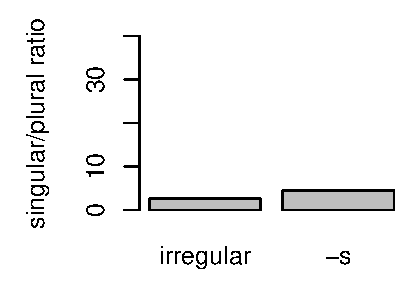
\includegraphics[width=\maxwidth]{figures/sramh-imgdisplay_epls_plot-1} 
\end{knitrout}
\todo[inline]{figure missing}
\end{figure}

Strikingly, the difference goes in the wrong difference here: irregular plurals are more frequent relative to their singular forms than regular \emph{-s} plurals with respect to their singular forms. This difference is significant: $t(90.318) = 3.151$, $p =  0.002$.

%library(lsr); cramersV()

We conclude that the distribution of irregular plurals is ambiguous. In terms of relative frequency of singulars and plurals, the distribution goes in the wrong direction. In terms of overall distribution, however, it goes in the right direction. There are 2891 instances of irregular plurals in Brown and 46083 instances of regular plurals. If we were to assume that both types were equally likely, the difference is certainly significant: $X^2(4344, N = 48974) = 425346.797$, $p < .001$.

\section{Zero marking}

Let's now turn to zero marking. The claim is that zero marking is more complex and therefore the prediction is that zero marking should be under-represented.

We examine this with respect to plurals in \e\ in the Brown corpus. Zero-marked plurals in \e\ includes examples like: \emph{deer}, \emph{aircraft}, \emph{buffalo}, etc. The difference in ratios between regular plurals in \emph{-s} and zero plurals is shown in Figure~\ref{fig:ezero}.

\begin{figure}
\caption{\del{Relative frequency of}\add{Singular-to-plural ratios for} regular and zero plurals in \e}
\label{fig:ezero}
\begin{knitrout}
\definecolor{shadecolor}{rgb}{0.969, 0.969, 0.969}\color{fgcolor}
% 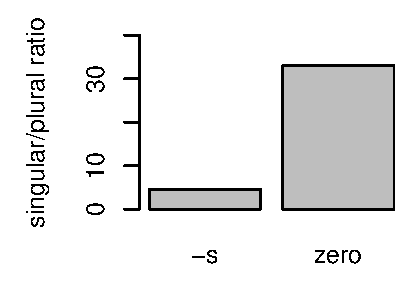
\includegraphics[width=\maxwidth]{sramh-imgdisplay_ezero_plot-1} 
\end{knitrout}
\todo[inline]{figure missing}
\end{figure}


Zero-marked plurals are far more frequent---relatively speaking---than regular plurals. Unfortunately, the variance is quite high\add{---there is a lot of variation within each category---}and though the mean difference is large, it is not significant: $t(19.002) = -1.416$, $p =  0.173$. As with the irregular plurals, however, the absolute difference is significant. There are 184 instances of zero plurals in Brown and 46083 instances of regular plurals. If we were to assume that both types were equally likely, the difference is certainly significant: $X^2(4285, N = 46267) = 311130.115$, $p < .001$. Again then, though the relative count is not significant, the absolute count goes in the right direction.

\section{Summary}

Our goal here has been to test the dimensions of morphological complexity proposed in \citet{dimensions} with the theory of \io. As reviewed above, \io\ maintains that grammatical complexity, as assessed through constraint violation, is minimized at the input level of the grammar. Specifically, we should see under-representation of more marked morphological structures.

We picked out several dimensions of morphological complexity to examine, some of which have already been treated with respect to \io. The following list is repeated from Section~\ref{sec:io} and annotated to reflect our results.

\begin{enumerate}

\item Words should have fewer \isi{morphemes}. \emph{This is borne out by the distribution of marked plurals and marked singulars in \w.}
%Welsh marked singulars vs. marked plurals

\item Haplology\is{haplology} should be avoided. (This has already been established by \citealt{inopt.phon}.)

\item More marked morphological operations (per the hierarchy above) should be avoided. \emph{This was tested with respect to \e\ plurals and is borne out in an absolute comparison, but not in a relative comparison.}
%ENG irreg plurals

\item Morphophonology should be avoided. (This has already been established by \citealt{inopt}.)

\item Ablaut, umlaut, truncation, etc.\ should be avoided. (This is essentially the same as \#3 above.)

\item Zero-marking should be avoided. \emph{This was tested with respect to \e\ plurals and is borne out in an absolute comparison, but not in a relative comparison.}
%ENG avoid plurals like sheep/deer/bear

\end{enumerate}

First, all else being equal, we expect forms with more morphemes to be dispreferred to forms with fewer morphemes. We saw that this was borne out in a comparison of singular--plural pairs in \w\ where in some cases the singular has an extra morpheme and in others the plural has an extra morpheme.

Second, we predict that morphological haplology should be under-represented. This was established in previous work with respect to the \e\ genitive plural and adjectives in \emph{-ly}.

Third, more marked morphological operations should be under-represented with respect to less marked morphological constructions. We saw an overall effect here with \e\ irregular noun plurals. We also saw that the relative distribution of plurals with respect to singulars went in the opposite direction.

Fourth, we predict that \isi{morphophonology} should be avoided. This was established in previous work with respect to morphophonology associated with \e\ past \emph{-ed} and plural \emph{-s}.

The fifth point is the same as the third.

Finally, zero-marking should be under-represented. We saw an overall effect here with \e\ zero-marked noun plurals. We also saw that the relative distribution of plurals with respect to singulars went in the opposite direction.

We conclude that the parameters of \isi{complexity} developed in \citet{dimensions} tested here and in previous work are correct.

We have seen that there is some divergence in the absolute and relative representation of plural marking, but we leave investigation of that for future work.

\section*{Acknowledgements}

Thanks to Nick Kloehn and Diane Ohala for useful discussion. All errors are my own.

\printbibliography[heading=subbibliography,notkeyword=this]


\end{document}
